Dans ce chapitre nous allons aborder les différents formats de données qui seront
et utilisés dans la suite de ce document.

\section{Nuage de point}
Un nuage de points est un ensemble de points de données dans un système de
coordonnées à trois dimensions. Il est généralement produit à partir d'un
instrument de \gls{lidar} ou en français détection et estimation de la distance
par la lumière. Il s'agit une technique de mesure de distance où la lumière réalise un 
aller-retour entre sa source et un objet. On chronomètre le temps entre le moment 
où une impulsion de lumière est émise par un laser et son retour vers un capteur.
En connaissant la vitesse de propagation de la lumière dans l’environnement où elle
évolue, il est possible de déterminer la distance qui sépare l’objet du capteur.
Plus précisément, il s’agit de la distance séparant le dispositif de mesure et
un point de l’objet frappé par la lumière émise. 
Cette opération effectuée à de multiples reprises en changeant par petit pas 
l’angle du laser, créer des points qui une fois réunis, constituent un nuage de points profilant l'environnement autour de l'instrument.
Si l'instrument de mesure est placé sur un aéronef et que la source de lumière est
dirigée vers le bas, il est ainsi possible de capturer, sous forme d'un nuage de
points, une région du globe. Ce cas nécessite de connaître la position
\gls{gps} du véhicule au moment de la capture d'un point afin de mettre en relation
tous les points à la fin de la mesure.
Il existe différentes versions de la spécification et ce document va se concentrer sur la version un point deux.

\subsection{Format LIDAR}
Le format de stockage des nuages de points de données \gls{lidar}, est un format
binaire dont les spécifications sont définies par l'\gls{asprs}.
Le format \gls{las} est composé de trois sections, respectivement:
L'en-tête de fichier, les enregistrements à longueur variable et les données liées aux points récoltés.

\begin{table}[!h]
    \centering
    \begin{tabular}{ |c|c| }
        \hline
        En-tête \\
        \hline
        Enregistrements à longueur variable \\
        \hline
        Données des points \\
        \hline
    \end{tabular}
    \caption[Sections composant un fichier au format LAS]{
            Sections composant un fichier au format LAS, 
            Source: adapté de LAS Specification Version 1.2 (2008, p. 2)
    }
    \label{tab:las_sections}
\end{table}
\newpage
Dans toutes les sections, on définit les types de données dans le tableau \ref{tab:data_type}
\begin{table}[htbp!]
    \centering
    \begin{tabular}{|l|c|}
    \hline
    \textbf{Type de donnée}           & \textbf{Nombre d'octets} \\ \hline
    char           & 1               \\ \hline
    unsigned  char & 1               \\ \hline
    short          & 2               \\ \hline
    unsigned short & 2               \\ \hline
    long           & 4               \\ \hline
    unsigned long  & 4               \\ \hline
    double \tablefootnote{selon le standard IEEE 754} & 8     \\ \hline
    \end{tabular}
    \caption[Type de données de la définition du format LAS]{
        Type de données de la définition du format LAS.
        Source: adapté de LAS Specification Version 1.2 (2008, p. 2-3)
    }
    \label{tab:data_type}
\end{table}

\subsection{En-tête public}

L'en-tête public comporte les métadonnées du fichier.
Il est composé de tous les champs du tableau~\ref {tab:las_header} présent dans l'annexe~1. Ils sont tous encodés en mode little endian.
Tous les champs inutilisés doivent être remplis par des bits nuls.
La signature de fichier doit obligatoirement contenir les quatre caractères “LASF” et celle-ci est requise par la spécification.
Un programme lisant le fichier doit vérifier cette signature pour déterminer qu’il s’agisse bien d’un fichier \gls{las}.

Parmi les champs, les facteurs $ X, Y $ et $ Z $ scale sont utilisés avec les valeurs $ X, Y$ et $Z$ offset pour obtenir des coordonnées cartésiennes des axes.
Ces valeurs sont globales au fichier. Voici la formule pour chaque coordonnée:

\begin{equation*}
    X_{coordinate} = (X_{record} * X_{scale}) + X_{offset}
\end{equation*}
\begin{equation*}
    Y_{coordinate}= (Y_{record} * Y_{scale}) + Y_{offset}
\end{equation*}
\begin{equation*}
    Z_{coordinate}= (Z_{record} * Z_{scale}) + Z_{offset}
\end{equation*}

Les champs min et max $X, Y, Z$ sont les valeurs minimales et maximales non mises à l'échelle des données des points présents dans la dernière section du fichier.

\subsection{Enregistrements à longueur variable}

Ce bloc suit directement l'en-tête public et peut avoir une ou plusieurs entrées.
Le nombre total d'entrées est spécifié dans le champ "Number of Variable Length Records" de l'en-tête.
Il doit être lu de manière séquentielle pour cause, la taille variable des données l'impose.
Chaque entrée est débutée par un en-tête de 54 octets selon le tableau \ref{tab:las_var_record_header}

\begin{table}[htbp!]
\centering
\begin{tabular}{|l|l|c|c|}
\hline
\multicolumn{1}{|c|}{\textbf{Champ}} & \multicolumn{1}{c|}{\textbf{Type de donnée}} & \textbf{Taille (Octets)} & \textbf{Requis} \\ \hline
Réservé                              & unsigned short                               & 2                        &                 \\ \hline
User ID                              & char{[}16{]}                                 & 16                       & *               \\ \hline
Record ID                            & unsigned short                               & 2                        & *               \\ \hline
Record Lenght After Header           & unsigned short                               & 2                        & *               \\ \hline
Description                          & char{[}32{]}                                 & 32                       &                 \\ \hline
\end{tabular}
\caption{
Champs de l'en-tête des enregistrements de longueur variable.
Source: adapté de LAS Specification Version 1.2 (2008, p. 6)}
\label{tab:las_var_record_header}
\end{table}

Les enregistrements peuvent provenir de sources différentes.
Elles sont identifiées par le champ "User ID" qui est une chaîne de caractères unique et enregistrée auprès d'un organe d'identification des producteurs de données lidar afin de prévenir que deux sources différentes aient la même séquence.

Chaque utilisateur dispose de 65536 enregistrements au maximum qu'il gère de manière indépendante.
Les identifiants des enregistrements sont renseignés dans le champ "Record ID" de l'en-tête.
Il peut également, s'il le souhaite, publier une signification liée aux identifiants choisis.

"Record Lenght After Header": il s'agit d'un offset en nombre d'octets qui indique l'endroit où commencent les données après l'en-tête de 55 octets.
La source des données peut renseigner des informations supplémentaires dans l'en-tête, mais elles ne suivront pas le standard de la spécification.

\subsection{Données des points}

Les données des points commencent à l'adresse du champ "Offset to Point Data" de l'en-tête de fichier.
Il existe quatre formats pour les entrées de point.

Le format zéro contient les champs communs à tous. Les informations présentées sont dans le tableau \ref{tab:las_point_data}
\begin{table}[htbp!]
\centering
\begin{tabular}{|l|l|c|c|}
\hline
\multicolumn{1}{|c|}{\textbf{Champ}}     & \multicolumn{1}{c|}{\textbf{Format de donnée}} & \textbf{Taille} & \textbf{Requis} \\ \hline
X                                        & long                                           & 4 octets        & *               \\ \hline
Y                                        & long                                           & 4 octets        & *               \\ \hline
Z                                        & long                                           & 4 octets        & *               \\ \hline
Intensity                                & unsigned short                                 & 2 octets        &                 \\ \hline
Return number                            & 3 bits (bits 0, 1, 2)                          & 3 bits          & *               \\ \hline
Number of returns (given pulse)          & 3 bits (bits 3, 4, 5)                          & 3 bits          & *               \\ \hline
Scan Direction Flag                      & 1 bit (bit 6)                                  & 1 bit           & *               \\ \hline
Edge of Flight Line                      & 1 bit (bit 7)                                  & 1 bit           & *               \\ \hline
Classification                           & unsigned char                                  & 1 octet         & *               \\ \hline
Scan Angle Rank (-90 to +90) – Left side & char                                           & 1 octet         & *               \\ \hline
User Data                                & unsigned char                                  & 1 octet         &                 \\ \hline
Point Source ID                          & unsigned short                                 & 2 octets        & *               \\ \hline
\end{tabular}
\caption{
Information d'un point présent dans un fichier \gls{las},
Source: adapté de LAS Specification Version 1.2 (2008, p. 6)}
\label{tab:las_point_data}
\end{table}

Les points sont collectés à partir des impulsions de laser envoyées et détecter par un capteur le tout depuis un aéronef.

Un exemple d'appareils est celui de la figure \ref{fig:lidar_scheme}

\begin{figure}[htbp!]
    \centering
    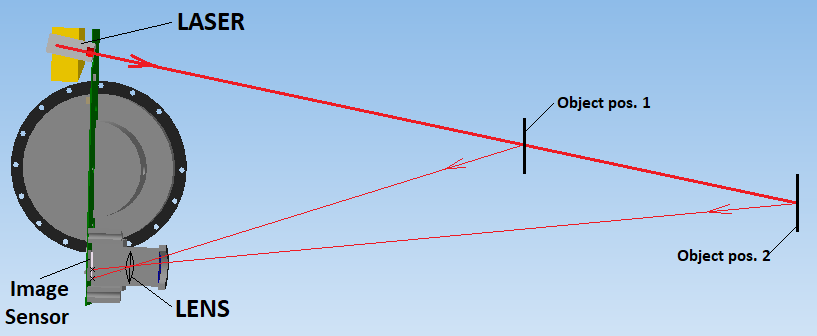
\includegraphics[width=0.8\linewidth]{figures/lidar_schema.png}
    \caption{Schéma représentant un instrument de mesure LIDAR. Source : tiré de réf URL02}
    \label{fig:lidar_scheme}
\end{figure}

On peut considérer une entrée dans le fichier comme une impulsion de lumière émise lors de la mesure des points.
Chaque impulsion peut recevoir plusieurs retours d'où le champ "Number of returns (given pulse)".
Il est aussi nécessaire de connaître l'angle de l'appareil par rapport à l'horizon afin de corriger la position du point récolté, car seul l'angle de l'instrument de mesure ne suffit pas.
Cet angle est en degré et allant de -90° à +90° à partir de l'aile gauche de l'aéronef dans le sens du vol.

Le format un ajoute simplement des informations concernant le temps \gls{gps} à laquelle le point a été enregistré.
Il est de même des autres format cependant ces informations ne sont pas utiles pour ce travail.

\subsection{Classification des points}

Les points collectés sont généralement classés selon le type de sol rencontré. Les valeurs se trouvent au tableau \ref{tab:las_point_class_meaning}.
Toutes les informations concernant le classement sont contenues en un octet et  en quatre sections. Elles sont expliquées dans le tableau \ref{tab:las_class_byte_explanation}.

Les cinq premiers bits correspondent à une table standard des classifications.
Si le bit cinq à un, le point a été créé par un logiciel de manière synthétique et si le bit sept est aussi à un, le point ne doit pas être pris en compte. Il est considéré comme étant supprimé.

\begin{table}[!h]
\centering
\begin{tabular}{ccccclll}
\hline
\multicolumn{1}{|c|}{0} & \multicolumn{1}{c|}{1} & \multicolumn{1}{c|}{2} & \multicolumn{1}{c|}{3} & \multicolumn{1}{c|}{4} & \multicolumn{1}{c|}{5}           & \multicolumn{1}{c|}{6}         & \multicolumn{1}{c|}{7}      \\ \hline
\multicolumn{5}{|c|}{N° de classification}                                                                                  & \multicolumn{1}{l|}{Synthétique} & \multicolumn{1}{l|}{Point clé} & \multicolumn{1}{c|}{Retenu} \\ \hline
\multicolumn{8}{c}{1 octet}                                                                                                                                                                                                  
\end{tabular}
\caption{ Représentation des bits dans l'octet de classification. Source : adapté de LAS Specification Version 1.2 (2008, p. 8)}
\label{tab:las_class_byte_explanation}
\end{table}

\begin{table}[htbp!]
\centering
\begin{tabular}{|c|l|}
\hline
\textbf{N° de classification (bit 0 à 4)} & \multicolumn{1}{c|}{\textbf{Signification}} \\ \hline
0                                         & Créé, jamais classé                         \\ \hline
1                                         & Non classé                                  \\ \hline
2                                         & Sol                                         \\ \hline
3                                         & Faible végétation                           \\ \hline
4                                         & Végétation moyenne                          \\ \hline
5                                         & Végétation dense                            \\ \hline
6                                         & Bâtiment                                    \\ \hline
7                                         & Bruit                                       \\ \hline
8                                         & Point de masse                              \\ \hline
9                                         & Eau                                         \\ \hline
10-11                                     & Réservé                                     \\ \hline
12                                        & Point superposé                             \\ \hline
13-31                                     & Réservé                                     \\ \hline
\end{tabular}
\caption{Signification des valeurs de classification. Source : adapté de LAS Specification Version 1.2 (2008, p. 8)}
\label{tab:las_point_class_meaning}
\end{table}

\section{Maillage}
Les maillages sont une modélisation géométrique d'un domaine spatial continu
par des éléments proportionnés finis.
Les maillages simplifient donc un système par un modèle représentant ce système
ou son environnement. Ils permettent notamment de réaliser des simulations ou bien d'avoir
une représentation graphique numérique.

\subsection{Fichier Stéréoligraphique}

Le format de \gls{stl} est conçu par la société 3D System pour contenir des maillages.
Il a été pensé pour permettre un prototypage rapide dans les logiciels de \gls{cao}. 
Ce format ne décrit que la géométrie de la surface d'un modèle.
Il existe un format binaire et un format ASCII, le dernier laissant une empreinte dans la mémoire morte plus conséquente.

On y stocke les triangles composant le modèle où chaque sommet du triangle est décrit par ses coordonnées cartésiennes $(x,y,z)$. Chaque triangle partage, sans exception, deux sommets avec un triangle voisin.
La coordonnée dans l'axe $z$ est considérée comme l'axe vertical, ceci peut être gênant pour les programmes considérant l'axe $y$ comme l'axe vertical.

\subsection{Format ASCII}

Le format commence par la séquence de caractères : "solid \textit{nom}" où \textit{nom} est une séquence correspondant au nom du modèle qui est facultatif.
Si le nom est vide, l'espace après "solid" est obligatoire.
Un triangle s'écrit de la manière suivante :
\begin{minipage}{\linewidth}
\begin{lstlisting}[frame=single, escapechar=\%]
facet normal % $n_x$% %$n_y$% %$n_z$%
    outer loop
        vertex %$v1_x$% %$v1_y$% %$v1_z$%
        vertex %$v2_x$% %$v2_y$% %$v2_z$%
        vertex %$v3_x$% %$v3_y$% %$v3_z$%
    endloop
endfacet
\end{lstlisting}
\end{minipage}
Les sommets sont définis à l'aide du mot clé "vertex" qui sont contenus dans un bloc loop. Les $n$ et les $v$ sont des nombres à virgule flottante.
Ils s'écrivent dans le format "signe-mantisse-e-signe-exposant", par exemple "6.248000e-003".
La fin du fichier ASCII est définie par la séquence : "end solid".

\subsection{Format binaire}

Le format binaire présente un avantage considérable par rapport au format ASCII, il est beaucoup moins volumineux. 

Les 80 premiers octets sont un commentaire. Les quatre suivants sont un entier 32 bits qui indique le nombre de triangles présent dans le fichier.
Chaque triangle est encodé sur 50 octets. Comme le format ASCII, les nombres sont encodés conformément à la spécification IEEE-754 et en mode little endian.

Le format dans le fichier est le suivant : 

\begin{lstlisting}[frame=single]
unsigned char[80] - header
unsigned int - total number of triangles

foreach triangle:
    float - normal vector
    float - vertex 1
    float - vertex 2
    float - vertex 3
unsigned short - control word
end
\end{lstlisting}